\chapter{Implementace}

\section{Použité nástroje}

Při návrhu metod jsem používal jazyk Python, který je vhodný pro analýzu dat, zvláště pak jeho knihovny NumPy, Pandas a SciPy pro zpracování a analýzu dat a matplotlib pro vykreslení dat. Dále jsem použil knihovny TensorFlow a Keras pro práci s neuronovými sítěmi a knihovnu Scikit-learn pro strojové učení.

Implementace modulů do SmartCGMS je v jazyce C++. Použití Keras modelu neuronové sítě je za pomoci knihovny frugally-deep\citep{cho.frugally}.

\section{Dataset BGLP}
\label{ch:bglp}

\begin{setlength}{\parskip}{0pt}
Anonymizovaná data ze senzoru CGMS obsahují naměřené a zadané hodnoty:
\begin{itemize}
\setlength\itemsep{0em}
\item Glukóza v krvi (BG)
\item Intersticiální glukóza (IST)
\item Bazální množství inzulinu
\item Bolus inzulinu
\item Příjem karbohydrátů (CHO)
\item Fyzická aktivita
\item Kvalita spánku
\item Elektrodermální aktivita
\item Teplota kůže
\item Teplota okolí
\item Srdeční tep
\item Počet kroků
\item Akcelerace
\end{itemize}
\end{setlength}

Intersticiální glukóza je měřena v pětiminutových intervalech. Glukóza v krvi, podávaný inzulin (bolus i bazál), karbohydráty, fyzická aktivita a kvalita spánku jsou zadávány pacientem. Senzor měří buď srdeční tep a počet kroků, nebo akceleraci. Srdeční tep a počet kroků se měří v pětiminutových intervalech, akcelerace v minutových intervalech. Elektrodermální aktivita a teplota kůže a okolí se měří ve stejném intervalu podle toho, zda se měří tep nebo akcelerace.

\begin{setlength}{\parskip}{0pt}
CGMS senzor posílá data ve formě signálů, které mají strukturu:
\begin{itemize}
\setlength\itemsep{0em}
\item Logical Clock
\item Device Time
\item Event Code
\item Signal
\item Info
\item Segment Id
\item Event Code Id
\item Device Id
\item Signal Id
\end{itemize}
\end{setlength}

Příklad signálů ze senzoru CGMS je v tabulce \ref{tab:cgms_data}. Informaci pro následnou detekci v sobě nesou sloupce Device Time (čas měření), Signal (typ signálu) a Info (hodnota).

\begin{table}[H]
\caption{Signály ze CGMS}
\label{tab:cgms_data}
\centering
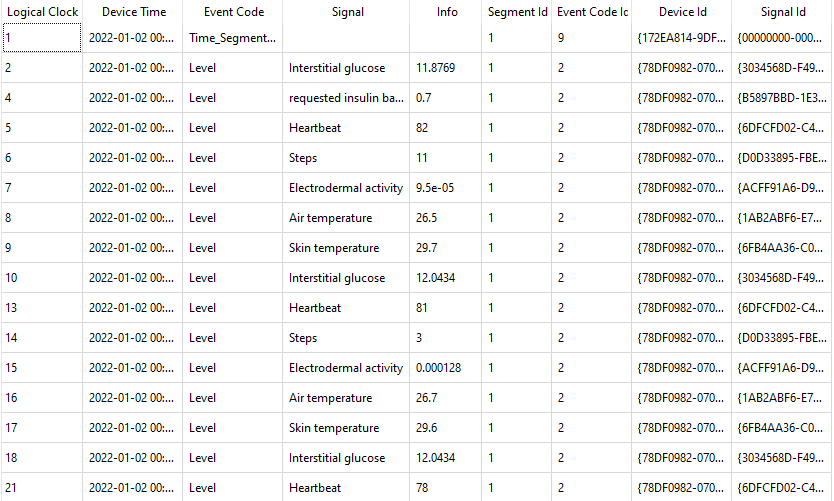
\includegraphics[width=1\textwidth]{img/cho/cgms_data.png}
\end{table}

V grafech na obrázku \ref{fig:48h_dataset} jsou transformovaná data naměřená senzorem CGMS za 48 hodin. Na prvním grafu jsou hodnoty Intersticiální glukózy a její vyhlazení Savitzky-Golay filtrem. Druhý graf znázorňuje zadanou bazální dávku inzulinu, bolusy, příjem karbohydrátů a fyzickou aktivitu. Na posledním grafu jsou hodnoty srdečního tepu, počtu kroků, elektrodermální aktivity, teploty kůže a teploty okolí.

\begin{figure}[H]
\caption{Data ze CGMS}
\label{fig:48h_dataset}
\centering
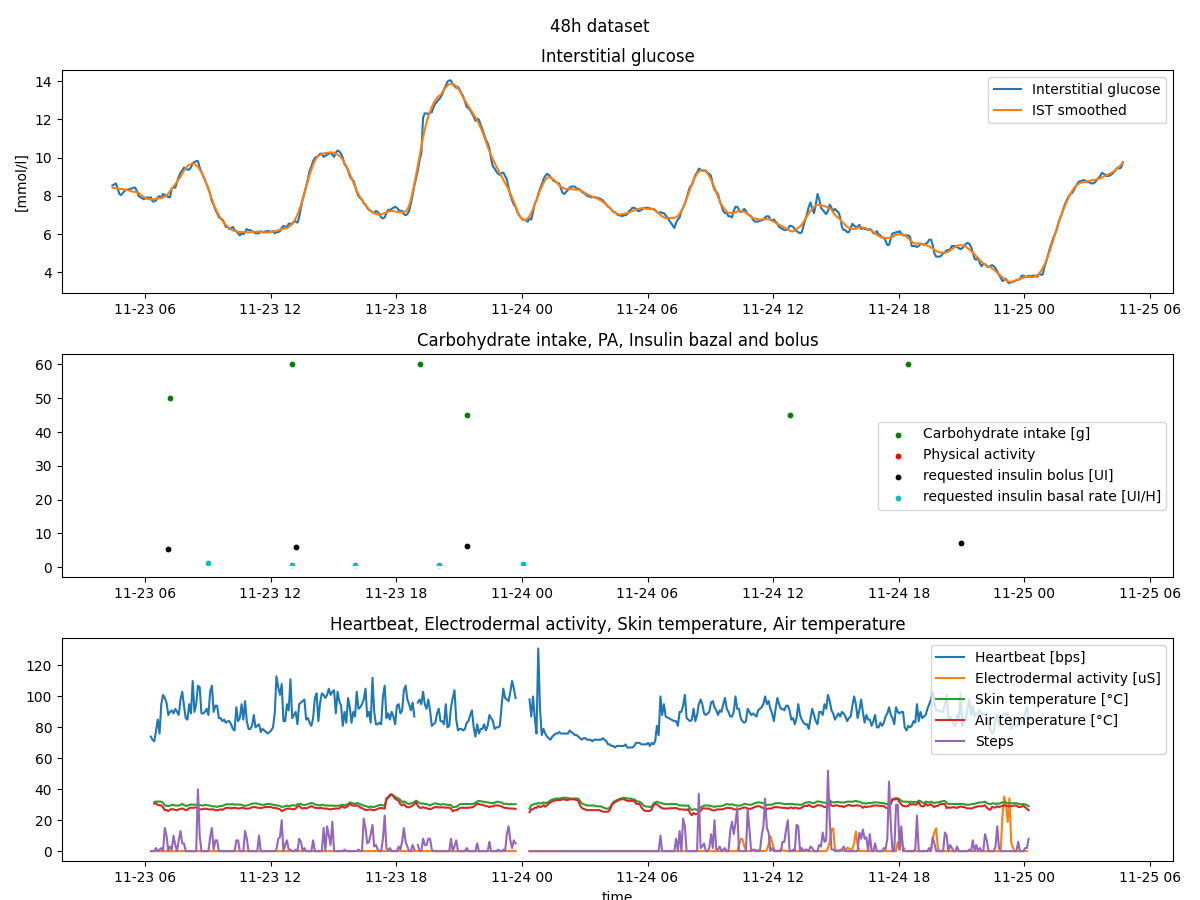
\includegraphics[width=1\textwidth]{img/cho/48h_dataset.png}
\end{figure}


\section{Filtr pro SmartCGMS}

Algoritmy jsou do SmartCGMS implementovány v podobě filtrů. Ty implementují rozhraní \textit{scgms::IFilter} a \textit{refcnt::IReferenced}. Při vytvoření instance filtru se volá metoda \textit{Configure}, která slouží pro nastavení filtru (typicky přečtení a nastavení konfiguračních parametrů). Metoda \textit{Execute} je volána pokaždé, když přijde signál od předchozího filtru. Tato metoda vykonává požadovanou funkcionalitu. Původní událost se na závěr zpravidla posílá dalšímu filtru. Současně se musí zaregistrovat descriptor nového filtru, který definuje ID filtru, název a konfigurační parametry, a případně i descriptor nového signálu. Vytvořená dynamická knihovna musí exportovat funkce \textit{do\_create\_filter}, \textit{do\_get\_filter\_descriptors} a \textit{do\_get\_signal\_descriptors}.

Data mohou být rozdělena do časových segmentů dle měření. V takovém případě filtry pracují s každým segmentem zvlášť. Rozdělení do segmentů je realizováno pomocí mapy, kdy klíčem je ID segmentu a hodnotou datová struktura pro daný filtr. Na konci segmentu se údaj z mapy vymaže.

Implementované algoritmy pracují s daty v určitém časovém okně. Pro tyto účely jsem vytvořil vlastní spojový seznam na principu klouzavého okénka \textbf{swl}. Ten dědí od \textit{std::deque}, které umožňuje vkládání prvků z obou stran i indexaci. Konstruktor má jeden parametr určující velikost okna. Při vložení nadlimitního prvků se odebere prvek z druhého konce seznamu.

Pro vyhlazení dat jsem implementoval \textbf{Savitzky-Golay} filtr. Tomuto filtru se nastavuje typ signálu, který má vyhladit, velikost okna a stupeň polynomu. Výstupem je \textbf{IST smoothed} signál.

Pro vyhodnocení úspěšnosti detekce je implementován \textbf{Evaluate} filtr. Tento filtr neřeší časové segmenty. Nastavit lze zkoumaný a referenční signál, časové okno pro detekci, cooldown pro započtení falešně pozitivního výsledku a minimální počet referenčních aktivit za den. Filtr započítává dvě úrovně detekovaného signálu. Nižší (1) pro detekované aktivity a vyšší (2) pro potvrzení. Filtr zaznamenává výsledky pro každý den. Pokud počet referenčního signálu je menší, než minimální počet, den se nezapočte do celkového součtu.

Možnosti nastavení všech filtrů a spuštění detekce je popsáno v příloze B.


\subsection{Detekce příjmu karbohydrátů}

\textbf{CHO detection} filtr počítá aktivační funkci a detekci karbohydrátů. To je implementováno rekurentní neuronovou sítí nebo detekcí hran průběhu intersticiální glukózy tak jak je popsáno v kapitole \ref{ch:threshold}. Filtr posílá dva signály. \textbf{Activation} signál je výstup použitého algoritmu a \textbf{CHO probability} udávající detekovaný příjem (1 - nižší pravděpodobnost, 2 - vyšší pravděpodobnost).

V případě detekce hran jsou nastaveny 2 thresholdy. Nižší pro brzkou detekci, která ale může detekovat výkyvy nesouvisející s příjmem jídla. Vyšší threshold je potvrzovací, kdy existuje vysoká pravděpodobnost příjmu karbohydrátů. Detekce je pouze pro vzestupnou hranu. Potvrzení může být i pomocí rekurentní neuronové sítě. Příklad konfigurace thresholdů je v konfiguračním souboru \texttt{setup\_th.ini} (viz příloha B). V případě detekce hran musí tomuto filtru předcházet Savitzky-Golay filtr pro vyhlazení dat intersticiální glukózy.

\subsubsection{Rekurentní neuronová síť}

Rekurentní neuronová síť využívá natrénovaného keras modelu.Ten je možné použít v C++ pomocí knihovny frugally-deep \citep{cho.frugally}.

Před trénováním modelu je třeba data ve formě signálů transformovat. Sloupce Device Time, Signal a Info jsem extrahoval do dvourozměrné tabulky, kde řádky jsou čas měření a sloupce jednotlivé typy signálů. Jelikož různé typy signálu nejsou měřeny ve stejný okamžik, řádky jsem seskupil podle sloupce intersticiální glukózy, která je měřena v pětiminutových intervalech. Data intersticiální glukózy jsem interpoloval Akima spline \citep{cho.akima}, z níž jsem získal chybějící hodnoty a derivace 1. 2. a 3. řádu.

Model může být natrénován individuálně pro každého pacienta, nebo na celém souboru dat. Vstupní data modelu jsou hodnoty intersticiální glukózy, jejich první derivace a čas signálu v minutách. Díky časovému údaji neuronová síť zahrne do predikce určité denní návyky pacienta. Časové okno je velikosti 24 (tj. 2 hodiny). Z datasetu je 80 \% dat použito pro trénování a 20 \% pro validaci. Data jsou do neuronové sítě dávkována v dávkách o velikosti 64. Jelikož se jedná o časovou řadu, data se nepromíchávají. Jako ztrátová funkce je použita střední kvadratická chyba (MeanSquaredError), optimalizační algoritmus je Adam. Neuronová síť je trénovaná ve 100 epochách. 

Natrénovaný model je nutné konvertovat pomocí skriptu \texttt{keras\_export/ convert\_model.py}, který je součástí frugally-deep knihovny. Podporované sítě jsou LSTM i GRU. SmartCGMS filtr následně tento model načte při konfiguraci. Příklad konfigurace s GRU je v konfiguračním souboru \texttt{setup\_gru.ini} (viz příloha B).



\subsection{Detekce fyzické aktivity}

Filtr \textbf{PA detection} detekuje fyzickou aktivitu na základě vybraných ukazatelů nebo jejich kombinace. Detekce probíhá z poslední hodnoty naměřené senzorem, nebo průměru více hodnot dle zvoleného časového okna. Pro každý ukazatel lze zadat threshold.

Pro detekci sestupné hrany je nutné před tento filtr zařadit \textit{Savitzky-Golay} filtr pro vyhlazení dat. Nastavení thresholdů a vah je stejné jako u detekce karbohydrátů.


V případě, že se nepoužívá potvrzení detekcí sestupné hrany, posílá filtr signál \textbf{PA detected} o hodnotě 2. Při použití detekce sestupné hrany má tento signál hodnotu 1 pokud byla aktivita detekována pouze na základě ukazatelů a hodnotu 2 pokud byla detekce potvrzena sestupnou hranou.

Příklad konfigurace s měřeným srdečním tepem a počtem kroků je v konfiguračním souboru \texttt{setup\_bpm.ini}. Příklad konfigurace s akcelerací a potvrzováním pomocí detekce sestupné hrany je v konfiguračním souboru \texttt{setup\_acc.ini} (viz příloha B).